\documentclass[10pt]{article}
\usepackage[utf8]{inputenc}
\usepackage[top= 0.3in]{geometry}
\usepackage{cite}
\title{Computação Musical e processamento de som: o backstage da produção musical correlacionada à tecnologia}
\author{Guilherme Macedo de Souza}
\date{31 de Outubro de 2019}

\usepackage{natbib}
\usepackage{graphicx}

\begin{document}

\maketitle

\section {Introdução}
\hspace{0.5in} A Computação Musical é uma interdisciplinalidade entre a música e as ciências da computação, dedicada ao estudo das aplicações dos computadores a problemáticas musicais. A computação musical investiga métodos, técnicas e algoritmos para processamento e geração sonora e acústica, representações digitais, e armazenamento de informação sonora. A computação musical lida com a forma de \textit{arte} ligada ao som, que tanto amamos: a música.
\begin{figure}[h!]
\centering
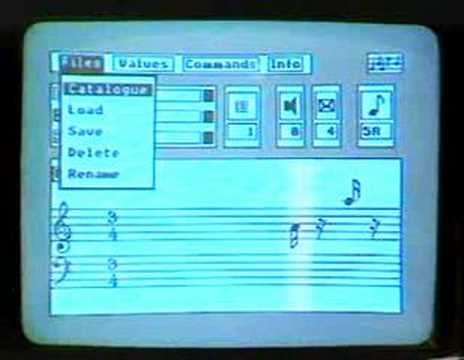
\includegraphics[scale=0.7]{hqdefault.jpg}
    \caption{Computer Music in 1985\hspace{0.02in}\cite{videocomputermusic}}
\label{fig:hqdefault}
\end{figure}
\section{Relevância}
\hspace {0.5in} A computação musical lida com a arte, tornando a disciplina um campo fértil para explorar a criatividade do aluno e relacionar com as técnicas de computação. Podemos exemplificar alguns métodos de uso da computação eletrônica em outras áreas:\begin{itemize}
    \item O uso de inteligências artificiais na fabricação musical\hspace{0.05in}\cite{miranda2013readings}\cite{ufpewebsite}
    \item Sistemas de educação musical e suas influências em áreas diversas, como reabilitação\hspace{0.05in}\cite{portaleducacaowebsite}
\end{itemize}

\section {Relação com outras disciplinas}
\hspace {0,5in} A disciplina de Computação Musical não possui outras disciplinas como pré-requisito. Porém, como toda área de conhecimento, ela usa outras áreas de conhecimento como alicerce. Como exemplo, temos:\begin{itemize}
    \item IF685 - Gerenciamento de Dados e Informação (GDI): o recebimento e armazenamento de dados é essencial, visto que é de necessidade prévia à conversão dos dados analógicos em digitais, e vice versa. Além disso, as ondas sonoras podem ser armazenadas e representadas como uma sucessão de números (dados) correspondentes às amplitudes do sinal, medidas a uma frequência constante.
    \item IF672 - Algoritmos e Estruturas de Dados: Visando agilidade na estruturação dos dados recebidos, a computação musical usa de algoritmos de compressão, podendo fazer com que um arquivo de áudio seja comprimido a 1/12 \hspace{0.01in}\cite{intromusical} do seu tamanho original.
    \item IF677 - Infraestrutura de Software: existem vários fabricantes de software para gravação de áudio digital, como a Digidesign (Pro Tools) e a Steinberg (Nuendo e Cubase). Além dos gravadores, existem os "samplers", que permitem gravar amostras e depois reproduzí-las com o auxílio da codificação de informação musical MIDI. Com o sampler, é possível gravar a voz com o microfone e disponibilizá-la sob a forma de um timbre, para ser executada por um teclado.
\end{itemize}
\bibliographystyle{plain}
\bibliography{gms4}
\end{document}
